%%%%%%%%%%%%%%%%%%%%%%%%%%%%%%%%%%%%%%%%%
% Memo
% LaTeX Template
% Version 1.0 (30/12/13)
%
% This template has been downloaded from:
% http://www.LaTeXTemplates.com
%
% Original author:
% Rob Oakes (http://www.oak-tree.us) with modifications by:
% Vel (vel@latextemplates.com)
%
% License:
% CC BY-NC-SA 3.0 (http://creativecommons.org/licenses/by-nc-sa/3.0/)
%
%%%%%%%%%%%%%%%%%%%%%%%%%%%%%%%%%%%%%%%%%

\documentclass[letterpaper,11pt]{texMemo} % Set the paper size (letterpaper, a4paper, etc) and font size (10pt, 11pt or 12pt)

\usepackage{fancyhdr}
\usepackage{fancybox}
\usepackage{longtable}
\usepackage{amsmath}
%----------------------------------------------------------------------------------------
%	MEMO INFORMATION
%----------------------------------------------------------------------------------------

\memoto{Luis Andr\'es Valido Fajardo. luis.valido@umcc.cu (53694742)} % Recipient(s)

\memofrom{Josval Díaz Blanco} % Sender(s)

\memosubject{Guía de Aprendizaje para Concursantes ICPC y IOI: Búsqueda Binaria } % Memo subject

\memodate{\today} % Date, set to \today for automatically printing todays date

\logo{
\includegraphics[scale=0.5]{img/icpc}} % Institution logo at the top right of the memo, comment out this line for no logo

%----------------------------------------------------------------------------------------

\begin{document}

%\AddToShipoutPicture{\BackgroundPic}
\maketitle % Print the memo header information
%\tableofcontents
\pagestyle{plain}
\pagebreak

\pagestyle{fancy}
\fancyhead[LO,CE]{ }
\fancyhead[RO,CE]{
\includegraphics[scale=0.1]{img/icpc}}
\fancyfoot[LO,CE]{\textbf{Autor:} Luis Andrés Valido Fajardo \\ \textbf{Email:} luis.valido1989@gmail.com \\ \textbf{Teléfono:} 53694742}
\fancyfoot[RO,CE]{\emph{Existen 10 tipos de personas Las que \\saben binario y LAS QUE NO}}
\fancypagestyle{plain}{\pagestyle{fancy}}



%\lhead{ }
%\rhead{  }

%\fancyfoot[L]{}
%\fancyfoot[R]{\textbf{Autor:} Luis Andrés Valido Fajardo \\ \textbf{Email:} luis.valido@umcc.cu}
%----------------------------------------------------------------------------------------
%	MEMO CONTENT
%----------------------------------------------------------------------------------------


\section{Introducción}
La distancia de edición o distancia de Levenshtein es el número mínimo de operaciones de edición necesarias para transformar una cadena en otra cadena. Las operaciones de edición permitidas son las siguientes:

\begin{itemize}
	\item Insertar un caracter( ABC $\rightarrow$ ABCA )
	\item Remover un caracter ( ABC $\rightarrow$ AB)
	\item Modificar un caracter ( ABC $\rightarrow$ ADC)
\end{itemize}

Por ejemplo, la distancia de edición entre LOVE y MOVIE es 2, porque primero podemos realizar la operación LOVE $\rightarrow$ MOVE (modificar) y luego la operación MOVE $\rightarrow$ MOVIE (insertar). Este es el menor número posible de operaciones, porque está claro que una sola operación no es suficiente.
\section{Conocimientos previos}
\subsection{Programación dinámica}
La programación dinámica es una técnica de optimización que se utiliza para resolver problemas complejos dividiéndolos en subproblemas más pequeños y resolviéndolos de manera recursiva. La idea principal detrás de la programación dinámica es almacenar los resultados de los
subproblemas resueltos para evitar repetir los cálculos y mejorar la eficiencia del algoritmo.

\subsection{Principio de óptimo}
Enunciado por Bellman en 1957 y que dice \emph{En una secuencia de decisiones óptima toda subsecuencia ha de ser también
óptima}. Hemos de observar que aunque este principio parece evidente no siempre es
aplicable y por tanto es necesario verificar que se cumple para el problema en
cuestión
\section{Desarrollo}
Supongamos que tenemos una cadena $x$ de longitud $n$ y una cadena $y$ de longitud $m$, y queremos calcular la distancia de edición entre $x$ e $y$.

Para resolver el problema utilizando programación dinámica es necesario
plantearlo como una sucesión de decisiones que satisfaga el principio de óptimo.
Para plantearla, vamos a fijarnos en el último elemento de cada una de las
cadenas. Si los dos son iguales, entonces tendremos que calcular el número de
operaciones básicas necesarias para obtener de la primera cadena menos el último
elemento, y la segunda cadena también sin el último elemento, es decir:

$$ distance(n,m) = distance(n-1,m-1) \quad \text{si} \quad x_n = y_m$$ 

Pero si los últimos elementos fueran distintos habría que escoger la situación
más beneficiosa de entre tres posibles: (i) considerar la primera cadena y la
segunda pero sin el último elemento, o bien (ii) la primera cadena menos el último
elemento y la segunda cadena, o bien (iii) las dos cadenas sin el último elemento.
Esto da lugar a la siguiente relación en recurrencia para $distance(n,m)$ para este caso:

$ distance(n,m) = 1 + \min \{ distance(n-1,m), distance(n,m-1),distance(n-1,m-1) \} \quad \text{si} \quad n\neq  0, m \neq  0, x_n \neq y_m $

En cuanto a las condiciones iniciales, tenemos las tres siguientes:

$$distance(0,0)=0, \qquad  distance(n,0)=n, \qquad distance(0,m)=m,$$

Una vez disponemos de la ecuación en recurrencia necesitamos resolverla
utilizando alguna estructura que nos permita reutilizar resultados intermedios.

Para resolver el problema, definimos una función $distance(a,b)$ que proporciona la distancia de edición entre prefijos $x[0 \dots a]$ y $y[0 \dots b]$. Por lo tanto, al usar esta función, la distancia de edición entre $x$ e $y$ es igual a la distancia ($n-1$,$m-1$).

Podemos calcular los valores de distancia de la siguiente manera:
$$
\begin{array}{cl}
distance ( a, b ) =	& min( distance ( a, b-1) + 1,  \\
	& distance ( a - 1, b ) + 1, \\
	& distance ( a - 1, b - 1) + cost ( a, b ))
\end{array}
$$



Aquí $cost( a, b ) = 0$ si $x[a]=y[b]$, y en caso contrario $cost(a,b)=1$. La fórmula considera las siguientes formas de editar la cadena $x$:

\begin{itemize}
	\item distance($a, b-1$): inserta un carácter al final de $x$.
    \item distance($a-1, b$): remueve el ultimo carácter de $x$.
    \item distance($a-1, b-1$): coincide o modifica el último carácter de $x$.
\end{itemize}

En los dos primeros casos, es necesaria una operación de edición (insertar o eliminar). En el último caso, si $x[a] = y[b]$, podemos hacer coincidir los últimos caracteres sin editar; de lo contrario, se necesita una operación de edición (modificar).

La siguiente tabla muestra los valores de distancia en el caso de ejemplo:

% TODO: \usepackage{graphicx} required
\begin{figure}[h!]
	\centering
	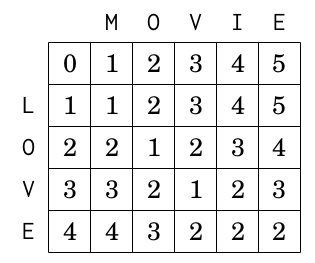
\includegraphics[width=0.3\linewidth]{img/edit_distance}
	\label{fig:editdistance}
\end{figure}


La esquina inferior derecha de la tabla nos dice que la distancia de edición entre LOVE y MOVIE es 2. La tabla también muestra cómo construir la secuencia más corta de operaciones de edición. En este caso el camino es el siguiente:

\begin{figure}[h!]
	\centering
	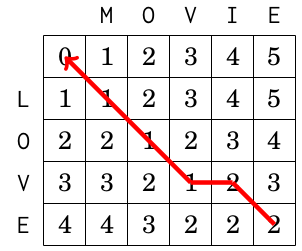
\includegraphics[width=0.3\linewidth]{img/edit_distance_2}
	\label{fig:editdistance2}
\end{figure}

Los últimos caracteres de LOVE y MOVIE son iguales, por lo que la distancia de edición entre ellos es igual a la distancia de edición entre LOV y MOVI. Podemos usar una operación de edición para eliminar el carácter I de MOVI. Por lo tanto, la distancia de edición es uno mayor que la distancia de edición entre LOV y MOV, etc.
\section{Implementación}
\subsection{C++}
\begin{lstlisting}[language=C++]
unsigned int edit_distance(string s1, string s2) {
   const size_t len1 = s1.size(), len2 = s2.size();
   vector< vector<unsigned int> > d(len1+1, vector <unsigned int>(len2 + 1));
   d[0][0] = 0;
   for (unsigned int i = 1; i <= len1; ++i) d[i][0] = i;
   for (unsigned int i = 1; i <= len2; ++i) d[0][i] = i;
	
   for (unsigned int i = 1; i <= len1; ++i)
      for (unsigned int j = 1; j <= len2; ++j)
         d[i][j] = min(min(d[i-1][j]+1,d[i][j-1]+1),
                       d[i-1][j-1]+(s1[i-1]== s2[j-1] ? 0 : 1));
   return d[len1][len2];
}
\end{lstlisting} 
\subsection{Java}

\begin{lstlisting}[language=Java]
public static int edit_distance(String s1, String s2) {
   int[][] dp = new int[s1.length()+1][s2.length()+1];
   for (int i = 0; i <= s1.length(); i++) dp[i][0] = i;
   for (int j = 0; j <= s2.length(); j++) dp[0][j] = j;
	
   for (int i = 1; i <= s1.length(); i++) {
      for (int j = 1; j <= s2.length(); j++) {
      	if (s1.charAt(i-1) == s2.charAt(j-1)) dp[i][j] = dp[i-1][j-1];
        else dp[i][j]= 1+ Math.min( Math.min( dp[i-1][j], dp[i][j-1]),
                                    dp[i-1][j-1]);
      }
   }
   return dp[s1.length()][s2.length()];
}
\end{lstlisting}


Nótese que $d[i-1][j]+1$ representa un costo de 1 para la inserción, $d[i][j-1]+1$
 costo 1 para eliminación, y $d[i-1][j-1]+(s1[i-1] == s2[j-1]? 0 : 1))$ representa
costo 1 para reemplazo (en caso de que no sean iguales). Con estas concideraciones
es fácil adaptar este problema a otros similares.
\section{Aplicaciones}
El cálculo de la distancia de edición, también conocida como distancia de Levenshtein, tiene diversas aplicaciones en diferentes campos. Algunas de estas aplicaciones incluyen:

\begin{enumerate}
	\item \textbf{Corrección ortográfica:} La distancia de Levenshtein se utiliza para sugerir correcciones para palabras mal escritas. Se compara la palabra ingresada con las palabras en un diccionario y se sugiere la palabra más cercana en términos de distancia de edición.
	\item \textbf{Búsqueda de similitud:} La distancia de edición se utiliza para encontrar la similitud entre dos cadenas de texto. Esto puede ser útil en la clasificación o agrupación de documentos basados en su similitud textual.
	\item \textbf{Algoritmos de autocompletar:} La distancia de Levenshtein se puede utilizar para implementar algoritmos de autocompletar en campos como los motores de búsqueda o los sistemas de entrada de texto predictivo en dispositivos móviles.
	\item \textbf{Comparación de secuencias genéticas:} La distancia de edición se utiliza en bioinformática para comparar secuencias genéticas y determinar su similitud o diferencia. Esto es útil en el estudio de la evolución genética y la identificación de relaciones entre diferentes especies.
	\item \textbf{Corrección gramatical:} La distancia de Levenshtein se puede utilizar para detectar errores gramaticales en oraciones y sugerir correcciones gramaticales adecuadas.
\end{enumerate}
\section{Complejidad}
El procedimiento descrito  va a permitir la creación de la tabla  que calcula el
número mínimo de operaciones básicas para la distancia de edición. La solución se encuentra en $[n,m]$, y la
 tabla se construye fila a fila (a partir de los valores que definen las condiciones
 iniciales) para poder ir reutilizando los valores calculados previamente. 
Como el algoritmo se limita a dos bucles anidados que sólo incluyen
operaciones constantes la complejidad de este algoritmo es de orden O($n\times m$) con similar complejidad espacial. Siendo $n$ y $m$ la longitud de las cadenas inciales. 
\section{Ejercicios}
A continuación una lista de ejercicios que se resuelven aplicando este algoritmo 

\begin{itemize}
	\item \href{https://cses.fi/problemset/task/1639/}{CSES - Edit Distance}
\end{itemize}

\end{document}